\section{Eprobung des Reglers an der Regelstrecke}
Der nächste Schritt besteht darin die Ergebnisse der letzten Abschnitte an der Regelstrecke zu erproben. Hierfür wird der in der Simulation optimierte Regler verwendet. Dieser führt zu den Eigenwerten
\begin{equation}
\begin{split}
\lambda_1 = 1 \hspace{15pt} \lambda_2 = 0{,}7714 \hspace{15pt} &\lambda_3 = 0{,}7767 \hspace{15pt} \lambda_4 = 0{,}8454
\\
\lambda_{5,6} = 0{,}8524\pm0{,}0014j \hspace{15pt} &\lambda_{7,8} = 0{,}8543 \hspace{15pt} \lambda_9 = 1 \,.
\end{split}
\label{eq_ew1_corner}
\end{equation}
Die folgenden Abbildung zeigen den Verlauf der Zustandsgrößen und der Stellgrößen.
\begin{figure}[h!]
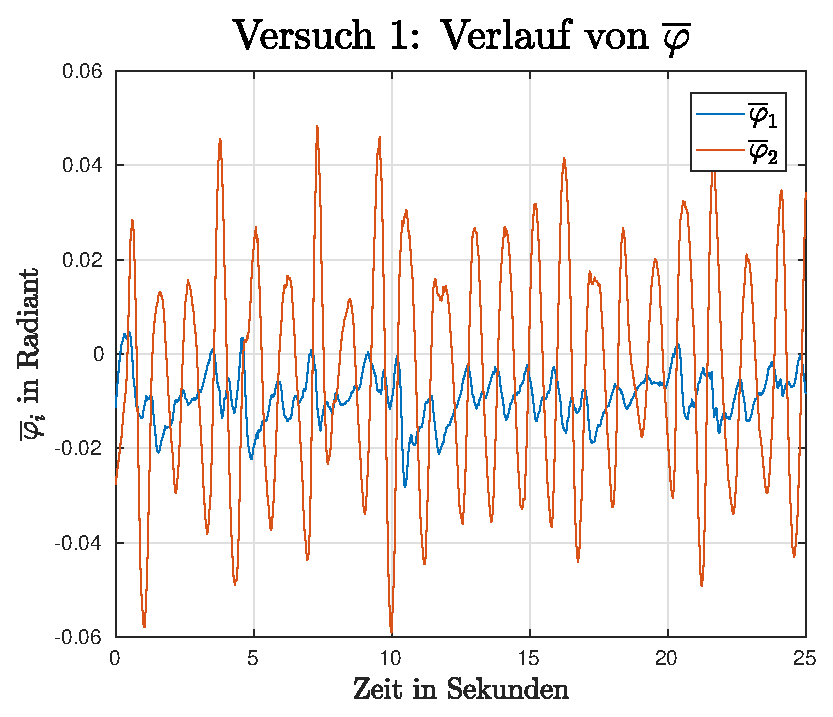
\includegraphics[width=0.45\linewidth]{img/exp1_phi.eps}
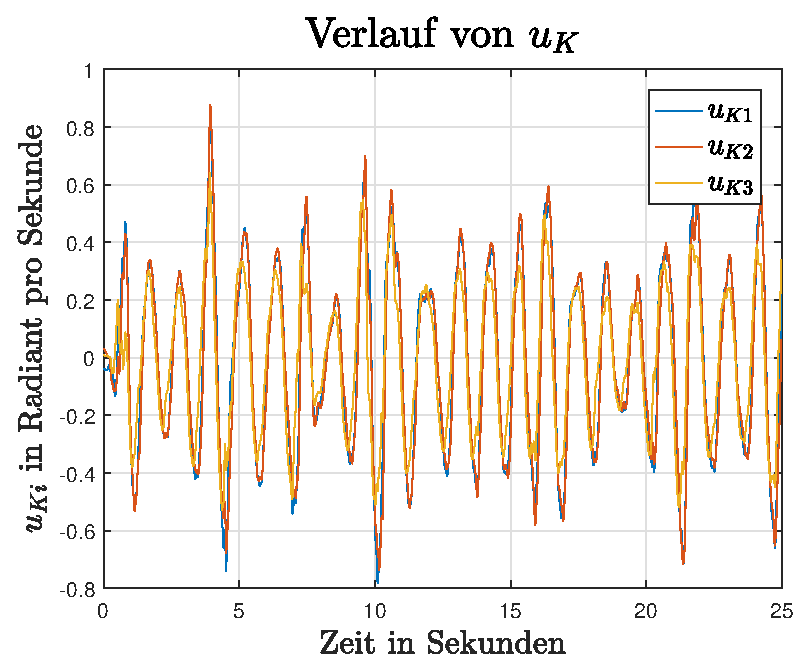
\includegraphics[width=0.45\linewidth]{img/exp1_uk.eps}
\vspace{0.5cm}

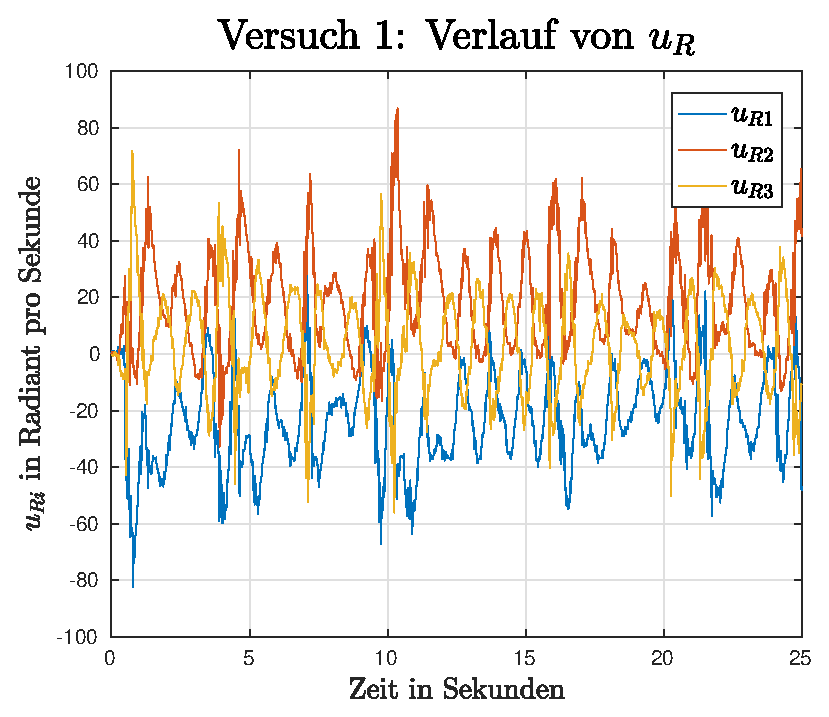
\includegraphics[width=0.45\linewidth]{img/exp1_ur.eps}
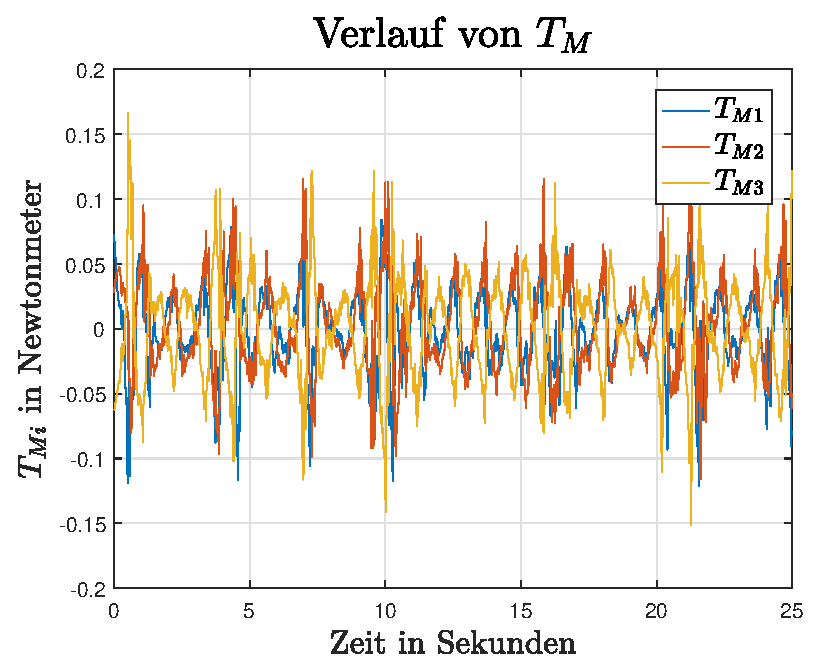
\includegraphics[width=0.45\linewidth]{img/exp1_tm.eps}
\caption{Systemverhalten des geschlossenen Regelkreises, Quelle: eigene Darstellung}
\end{figure}
Das Experiment zeigt, dass der Regler den Würfel auf einer Ecke stabilisiert. Allerdings ist das System nicht asymptotisch stabil sondern oszilliert mit einer konstanten Amplitude. Eine mögliche Erklärung für diese Verhalten liegt in der Modellgüte. Um die Direktionalitätsproblematik zu lösen wurde ein Regler gewählt, welcher die Eigenwerte des geschlossenen Kreises nahe an den Einheitskreis legt. Sind nun die Systemparameter des Modells fehlerbehaftet ist es möglich, dass die Eigenwerte des realen Regelkreises noch näher an dem Einheitskreis liegen. In diesem Fall können bereits kleinen Anregungen wie z.B. ein im Modell nicht erfasstes System- oder Messrauschen zu einer verbleibenden Schwingung führen. Des weiteren ist der Einfluss der Nichtlinearitäten zu nennen, welche die Auswirkungen der Modellungenauigkeiten zusätzlich beeinflussen können. 

Um die Reglergüte zu verbessern werden zunächst die Versuchsergebnisse betrachtet. Besonders deutlich ist einerseits die Schwingung des Winkels $\varphi_3$. Des weiteren sind die Signale $u_{Ki}(t)$ nahezu identisch. Dies entspricht einer Rotation des Würfels um seine Raumdiagonale. Um diese Oszillationen zu dämpfen werden einzelne Elemente der Reglermatrix schrittweise erhöht und die Veränderung empirisch überprüft. Die veränderten Elemente sind einerseits die Spalte $\bs{K}(:,3)$, welche den Einfluss des Winkels $\varphi_3$ auf den Regler wiedergibt. Andererseits wurden die Elemente $\bs{K}(1,4)$, $\bs{K}(2,5)$ und $\bs{K}(3,6)$ erhöht, welche den Einfluss der Winkelgeschwindigkeit in Richtung der Raumdiagonalen wiedergeben. Die Erhöhung dieser Elemente führt dazu, dass die Eigenwerte der zugehörigen Eigenbewegungen näher an den Ursprung gerückt werden. Die folgenden Abbildungen zeigen das Verhalten des geschlossenen Regelkreises, wobei die genannten Elemente der Reglermatrix um den Faktor zwei erhöht wurden.
\begin{figure}[h!]
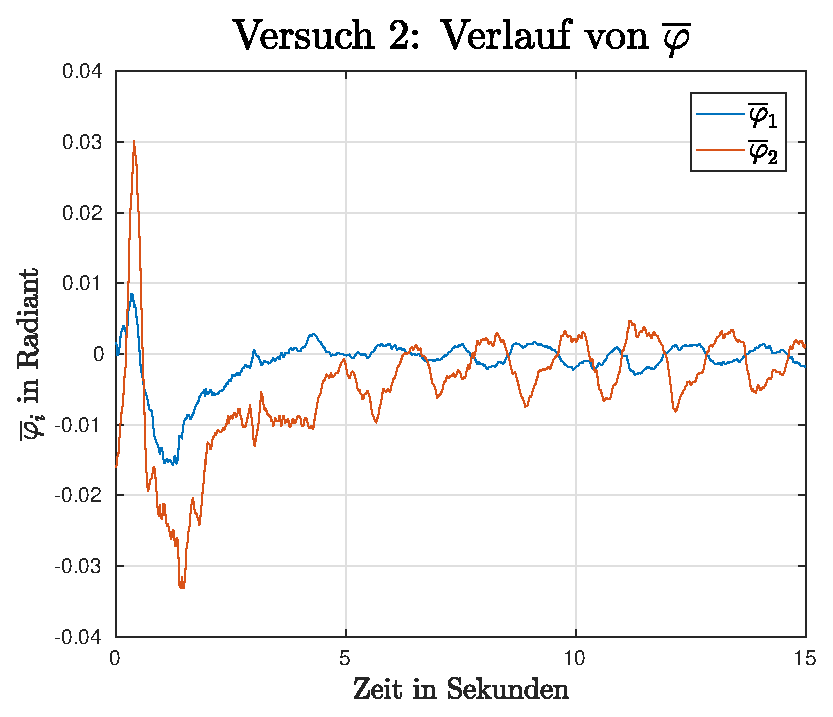
\includegraphics[width=0.45\linewidth]{img/exp2_phi.eps}
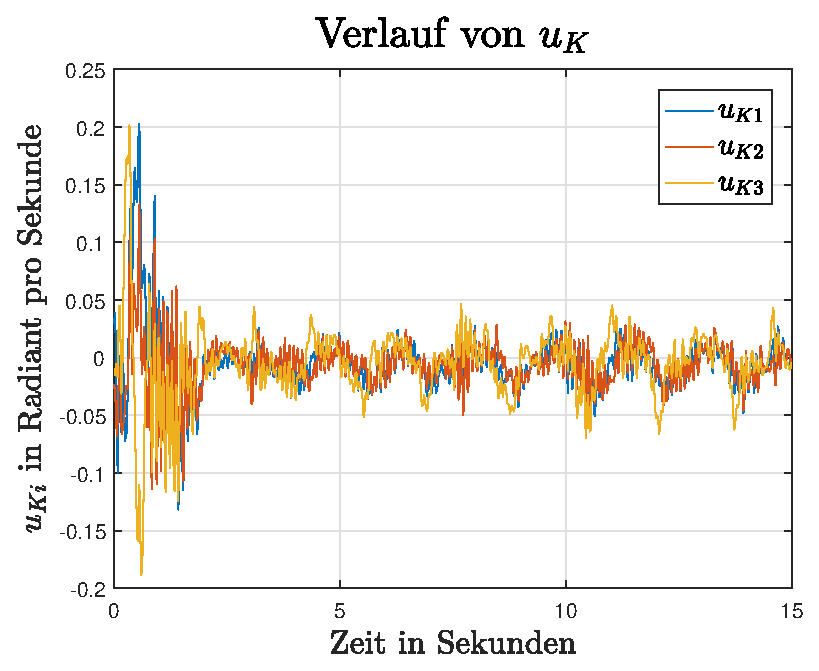
\includegraphics[width=0.45\linewidth]{img/exp2_uk.eps}
\vspace{0.5cm}

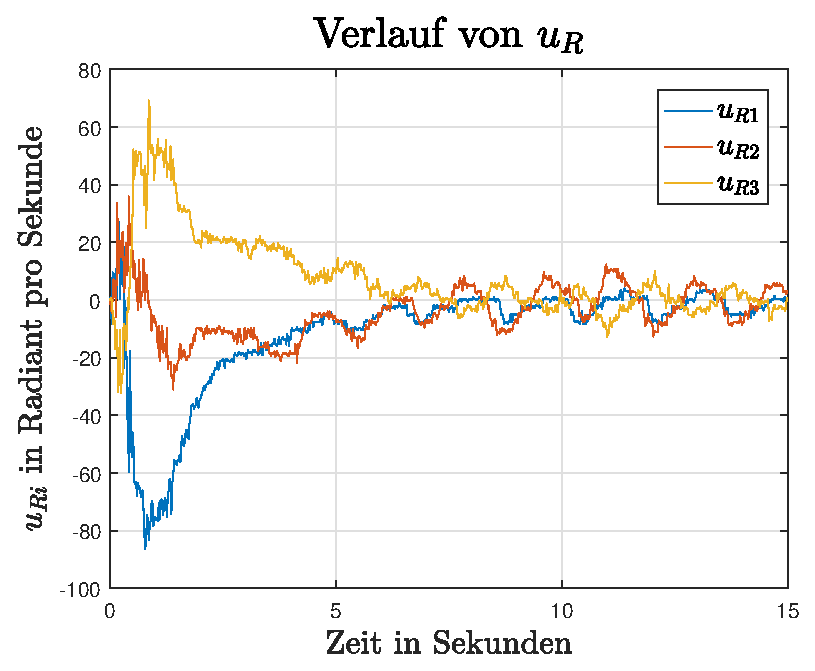
\includegraphics[width=0.45\linewidth]{img/exp2_ur.eps}
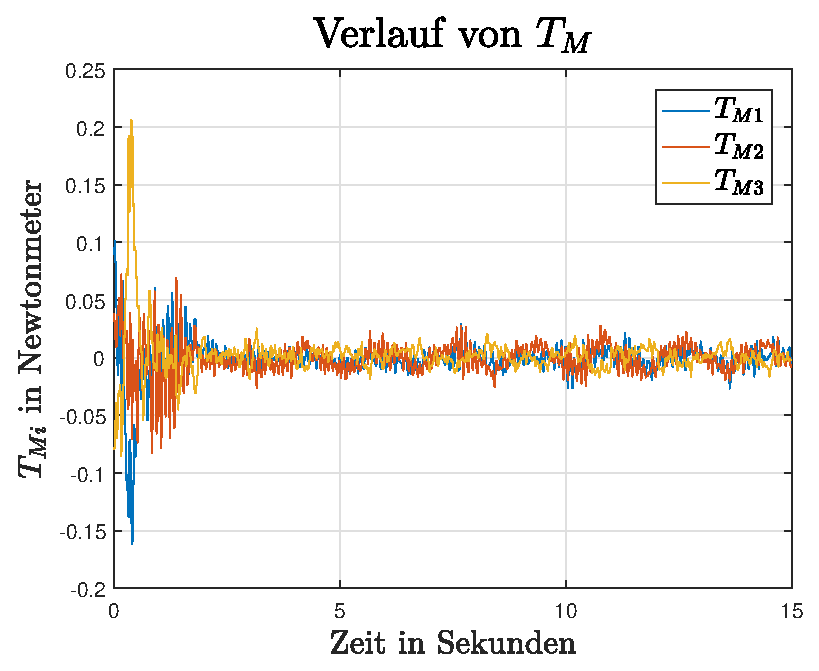
\includegraphics[width=0.45\linewidth]{img/exp2_tm.eps}
\caption{Verhalten des geschlossenen Regelkreises mit angepasstem Regler, Quelle: eigene Darstellung}
\end{figure}
Aus den Versuchen geht hervor, dass die Anpassung des Reglers eine deutliche Verbesserung des geschlossenen Regelkreises mit sich bringt. Jedoch ist diese Vorgehensweise kritisch zu beurteilen. Einerseits verbleibt eine Schwingung, welche ähnlich zu dem Verhalten aus dem vorherigen Versuch ist. Lediglich die Amplitude der Schwingung wurde die Änderung der Reglermatrix reduziert. Andererseits führt der Eingriff in die Reglermatrix dazu, dass die Reglereigenschaften, welche aus dem LQR-Verfahren resultieren, nicht mehr garantiert werden. Insbesondere die guten Robustheitseigenschaften können verloren gehen. Dies zeigt sich wenn die Reglerelemente weiter verändert werden um die verbleibenden Schwingungen zu eliminieren. Derartige Änderungen führen zu einem instabilen Regelkreis.

Der erste Schritt um diese Probleme zu beseitigen besteht darin eine Systemidentifikation durchzuführen. Der Grund wieso dies bisher nicht erfolgt ist liegt darin, dass kein Versuchsaufbau vorliegt an dem die Identifikation durchgeführt werden kann. Da hier lediglich diskretisierte Systeme der Regelstrecke betrachtet werden, entsprechen die Elemente der System- und Eingangsmatrix keinen physikalischen Größen wie z.B. einem Trägheitsmoment. Beispielsweise ist es schwierig eine Systemidentifikation des auf einer Kante balancierenden Würfels durchzuführen und die Ergebnisse auf diesen Anwendungsfall zu übertragen. Es bestehen zwar Methoden für die Parameterschätzung kontinuierlicher Regelstrecken [Unbi], allerdings sind diese mit zusätzlichen Problemen verbunden. Des weiteren ist es schwierig einen Versuchsaufbau zu entwickeln mit dem sämtliche Parameter des auf der Ecke stehenden Würfels identifiziert werden können.

Jedoch ermöglicht der hier präsentierte Regler eine Systemidentifikation. Hierfür können Parameterschätzverfahren für geschlossene Regelkreises angewandt werden [Unbi]. Diese basieren darauf das Modell des offenen Regelkreises zu betrachten und dessen Eingangssignal aus der Summe des Reglergesetzes und eines Testsignals zu berechnen. Durch den Regler ist das System stabil, wodurch die Identifikation möglich wird. Als Testsignal kann beispielsweise eine harmonische Schwingung verwendet werden, derer Frequenz variiert wird um das vollständige Übertragungsverhalten des Systems abzudecken [Unbi]. Mit diesem Versuchsaufbau kann zunächst die diskrete Übertragungsfunktionmatrix der Regelstrecke bestimmt werden, welche dem Unterraum der Minimalrealisierung \textfrak{D}$_M$ entspricht. Des weiteren können die Amplituden der Testsignale variiert werden um die Auswirkungen der Nichtlinearitäten abzuschätzen [Unbi]. An Hand der Ergebnisse der Systemidentifkation können anschließend weitere Verbesserungen an dem Regler durchgeführt werden.